%\immediate\write18{tex penrose_code.dtx}
\documentclass{ltxdoc}
\usepackage[T1]{fontenc}
\usepackage{trace}
\usepackage{lmodern}
\usepackage{morefloats}
\usepackage{multicol}
\usepackage[svgnames]{xcolor}
\usepackage{tikz}
\usetikzlibrary{
  external,
  tilings.polykite,
  tilings.penrose
}

\usepackage[numbered]{hypdoc}
\definecolor{lstbgcolor}{rgb}{0.9,0.9,0.9} 
 
\usepackage{listings}
\lstloadlanguages{[LaTeX]TeX}
\lstset{
  breakatwhitespace=true,
  breaklines=true,
  language=[LaTeX]TeX,
  basicstyle=\small\ttfamily,
  keepspaces=true,
  columns=fullflexible
}

\usepackage{fancyvrb}

\newenvironment{example}
  {\VerbatimEnvironment
   \begin{VerbatimOut}{example.out}}
  {\end{VerbatimOut}
   \begin{center}
   \setlength{\parindent}{0pt}
   \fbox{\begin{minipage}{.9\linewidth}
     \lstinputlisting[]{example.out}
   \end{minipage}}

   \fbox{\begin{minipage}{.9\linewidth}
     \centering
     \input{example.out}
   \end{minipage}}
\end{center}
}

\newenvironment{justexample}
  {\VerbatimEnvironment
   \begin{VerbatimOut}{example.out}}
  {\end{VerbatimOut}
   \begin{center}
   \setlength{\parindent}{0pt}
   \fbox{\begin{minipage}{.9\linewidth}
     \lstinputlisting[]{example.out}
   \end{minipage}}
\end{center}
}

\colorlet{thinRhombus}{DarkOrchid}
\colorlet{thickRhombus}{DarkSlateGray}
\colorlet{circleArc}{RosyBrown}
\colorlet{longArc}{LawnGreen}

\colorlet{kite}{HotPink}
\colorlet{dart}{Fuchsia}

\colorlet{goldenTriangle}{Gold}
\colorlet{reverseGoldenTriangle}{Magenta}
\colorlet{goldenGnomon}{Cyan}
\colorlet{reverseGoldenGnomon}{LimeGreen}

\makeatletter
\tikzset{
  tint fill colour/.code={%
    \edef\@temp{%
      \def\noexpand\tikz@fillcolor{\tikz@fillcolor!#1}%
      \noexpand\tikz@addoption{\noexpand\pgfsetfillcolor{\tikz@fillcolor!#1}}%
    }%
    \@temp
  }
}
\makeatother

  \tikzexternalize
  \tikzsetexternalprefix{penrose-doc-}
  
\providecommand*{\url}{\texttt}
\GetFileInfo{tikzlibrarytilings.code.tex}

\title{The \textsf{Tilings} Package: Documentation}
\author{Andrew Stacey\texorpdfstring{\\ \url{loopspace@mathforge.org}}{}}
 \date{\fileversion~from \filedate}

\begin{document}

\maketitle

\tableofcontents
  
\section{Introduction}

The \textsf{Tilings} package is a TikZ library for drawing tiles and tilings, such as Penrose tilings.
It currently supports natively the various Penrose tile sets -- kite/dart, rhombus, and pentagon -- and the aperiodical polykites, but has provision for defining new tiles.
There are two main methods for their placement: one that automatically generates a tiling, and one that allows for ``by hand'' placement.
Furthermore, the tiles themselves can be deformed and will still (hopefully!) fit together in the correct fashion.

\section{Initialisation}

This is actually several libraries.
There is a core library called \Verb+tilings+ which defines the main functionality for working with tiles and tilings but which doesn't define any tiles itself.
For that, there are currently two sublibraries:
%
\begin{itemize}
\item \Verb+tilings.penrose+ for Penrose tiles,
\item \Verb+tilings.polykite+ for the aperiodical polykite tiles.
\end{itemize}
%
The sublibraries automatically load the core library.

So to use this package, load the \Verb+tikz+ package and load one of the tilings libraries as a TikZ library.
Specifically, your preamble should contain:

\begin{verbatim}
\usepackage{tikz}
\end{verbatim}

\noindent and at least one of the following lines:

\begin{verbatim}
\usetikzlibrary{tilings}
\usetikzlibrary{tilings.penrose}
\usetikzlibrary{tilings.polykite}
\end{verbatim}

The original version of this package concerned itself only with Penrose tiles so was named \Verb+penrose+.
Since then it has been extended and is more general and so has been renamed \Verb+tilings+.
Some commands have been renamed, but there is a wrapper library which aims to provide backwards compatibility with the original naming scheme.
This is now the \Verb+penrose+ TikZ library, meaning that old documents that use the \Verb+penrose+ TikZ library should still work (please report any that don't on the \href{https://github.com/loopspace/penrose}{issue tracker}).
New documents shouldn't be written using it.


\section{Defining the Tiles}

This package includes the capability to define new tiles.
The command to do this is:
%
\begin{verbatim}
\DefineTile{<name>}{<sides>}{<vertices>}
\end{verbatim}
%
For example,
%
\begin{verbatim}
\DefineTile {square}{a A a A}
{
  {0,0}
  {1,0}
  {1,1}
  {0,1}
}
\end{verbatim}

The \Verb!<sides>! is a list of letters representing sides for matching rules and positioning.
The first letter in the list corresponds to the edge between the first two vertices, through to the last side which corresponds to the edge between the last and first vertices.

Each letter used matches against its opposite case (so it is possible to create a side that matches against itself by using a symbol that \TeX\ regards as having the same upper as lower case; not all symbols work, I've used numbers and \Verb+!+ successfully).
These are also used in path replacing, both a letter and its opposite case are replaced by the corresponding path (but in opposite directions) when the tile is ``baked''.

The vertices can be written in cartesian form: \Verb+{<x>,<y>}+, or in polar: \Verb+{<angle>:<length>}+ (with the angle in degrees).
The vertex can be preceded by upto two \Verb!+! signs which have the same interpretation as in TikZ: the vertex description is taken relative to the previously saved point with a single \Verb!+! additionally not updating the last saved point.
The initial saved point is the origin, so the following defines a hexagonal tile.
%
\begin{verbatim}
\DefineTile {hexagon}{a A a A a A}
{
  +{0:1}
  +{60:1}
  +{120:1}
  +{180:1}
  +{240:1}
  +{300:1}
}
\end{verbatim}

The numbers are passed to the \Verb!fp! module of \LaTeX3 so can involve complicated expressions.
Note that the trigonometric functions for angles in degrees are \Verb!cosd!, \Verb!sind!, and \Verb!tand!.

The tile must be baked via the command \Verb!\BakeTile! before it can be used.

\begin{example}
\DefineTile {square}{a A a A}
{
  {0,0}
  {1,0}
  {1,1}
  {0,1}
}

\begin{tikzpicture}
\path[save tiling path=a] (0,0) to[out=45,in=135] (1,0);
\BakeTile{square}
\pic[square,name=A,fill=green];
\pic[square,align with=A along a1 using 2,name=B,fill=red];
\pic[square,align with=A along A1 using 2,fill=red];
\pic[square,align with=A along A2 using 1,fill=red];
\pic[square,align with=B along a1 using 2,fill=green];
\pic[square,align with=B along a2 using 1,fill=green];
\end{tikzpicture}
\end{example}

\subsection{Predefined Tiles: Penrose}

The sublibrary \Verb+tilings.penrose+ defines a slew of tiles based on Penrose tilings.

\tikzset{
  every tile pic/.style={draw,ultra thick},
  every circle arc/.style={draw,thin},
  every long arc/.style={draw,thin},
}

\begin{itemize}
\item Kite \tikz[baseline=-.5ex] \pic[draw,kite];
\item Dart \tikz[baseline=-.5ex] \pic[draw,dart];
\item Thin Rhombus \tikz[baseline=-.5ex] \pic[draw,thin rhombus];
\item Thick Rhombus \tikz[baseline=-.5ex] \pic[draw,thick rhombus];
\item Pentagon \tikz[baseline=-.5ex] \pic[draw, pentagon 5];
(Actually, there are three pentagons: \Verb+pentagon 5+, \Verb+pentagon 3+, and \Verb+pentagon 2+.
The number signifies how many pentagons it goes next to.)
\item Pentagram \tikz[baseline=-.5ex] \pic[draw, pentagram];
\item Boat \tikz[baseline=-.5ex] \pic[draw, boat];
\item Diamond \tikz[baseline=-.5ex] \pic[draw, diamond];
\item Golden Triangle \tikz[baseline=-.5ex] \pic[draw,golden triangle];
\item Reverse Golden Triangle \tikz[baseline=-.5ex] \pic[draw,reverse golden triangle];
\item Golden Gnomon \tikz[baseline=-.5ex] \pic[draw,golden gnomon];
\item Reverse Golden Gnomon \tikz[baseline=-.5ex] \pic[draw,reverse golden gnomon];
\end{itemize}

The main tiles can have arcs drawn on them to illustrate the matching rules.
The triangles and gnomon are not true Penrose tiles but rather can be used to build tilings so they do not have the arcs.
The two types of each triangle and gnomon are actually different in that they have different matching rules.
This is best illustrated by deforming the paths (see Section~\ref{sec:pathdeform}).

The edge labelling is as follows.
For the \Verb+pentagon 5+, for example, the edges are all the same and the numbers are used to distinguish between them.

\begin{multicols}{2}

\foreach \tile/\edges in {
  kite/{a,A,c,C},
  dart/{a,A,c,C},
  thin rhombus/{a,A,b,B},
  thick rhombus/{a,A,b,B},
  pentagon 5/{a1,a2,a3,a4,a5},
  pentagon 3/{A,b1,a1,a2,b2},
  pentagon 2/{d,A1,e,c,A2},
  pentagram/{C1,E1,C2,E2,C3,E3,C4,E4,C5,E5},
  boat/{C1,E1,C2,E2,B1,D,B2},
  diamond/{D1,B1,B2,D2},
  golden triangle/{a,b,c},
  reverse golden triangle/{A,B,C},
  golden gnomon/{A,b,C},
  reverse golden gnomon/{a,B,c}} {

\begin{tikzpicture}
\pic[draw,\tile,name=tile];
\foreach \e in \edges {
    \path (tile-edge \e\space start) -- node[fill=white,fill opacity=.5,text opacity=1] {\e} (tile-edge \e\space end);
}
\end{tikzpicture}

}

\end{multicols}

\subsection{Predefined Tiles: Polykite}

The sublibrary \Verb+tilings.polykite+ defines a slew of tiles based on the aperiodical polykite tilings as described in \href{https://arxiv.org/abs/2303.10798}{An Aperiodic Monotile}.
It also defines a wrapper around the \Verb+\DefineTile+ command for creating one of the family of polykite tiles described in that article:

\begin{verbatim}
\DefinePolykiteTile{<name>}{<a>}{<b>}
\DefinePolykiteTile{aperiodical hat}{sqrt(3)/2}{1/2}
\end{verbatim}

(Note that the aperiodical hat tile is already defined.)

\begin{itemize}
\item Aperiodical Hat \tikz[baseline=-.5ex] \pic[draw,aperiodical hat];
\item Aperiodical Turtle \tikz[baseline=-.5ex] \pic[draw,aperiodical turtle];
\item Meta Cluster H \tikz[baseline=-.5ex] \pic[scale=.5,draw,meta cluster H];
\item Meta Cluster F \tikz[baseline=-.5ex] \pic[scale=.5,draw,meta cluster F];
\item Meta Cluster T \tikz[baseline=-.5ex] \pic[scale=.5,draw,meta cluster T];
\item Meta Cluster P \tikz[baseline=-.5ex] \pic[scale=.5,draw,meta cluster P];
\item Super Cluster H \tikz[baseline=-.5ex] \pic[scale=.3,draw,super cluster H];
\item Super Cluster F \tikz[baseline=-.5ex] \pic[scale=.3,draw,super cluster F];
\item Super Cluster T \tikz[baseline=-.5ex] \pic[scale=.3,draw,super cluster T];
\item Super Cluster P \tikz[baseline=-.5ex] \pic[scale=.3,draw,super cluster P];
\item Subcluster H \tikz[baseline=-.5ex] \pic[scale=.5,draw,subcluster H];
\item Subcluster F \tikz[baseline=-.5ex] \pic[scale=.5,draw,subcluster F];
\item Subcluster T \tikz[baseline=-.5ex] \pic[scale=.5,draw,subcluster T];
\item Subcluster P \tikz[baseline=-.5ex] \pic[scale=.5,draw,subcluster P];
\end{itemize}

The edges of the meta and super cluster tiles are actually multi-edges for the matching rules.

The subcluster tiles are a bit different to the others.
The \(H\) and \(T\) tiles are actually equilateral triangles but they have edge deformations applied by default so that they have the appearance of the aperiodical hat tile.
The \(P\) and \(F\) tiles have no area (so are not clipped by default) which means that the edge labels aren't fully clear as to which side they are on.
They match the diagrams given in the \href{https://arxiv.org/abs/2303.10798}{paper}, with the \(L\) sides being the sides labelled \(11\) and \(12\). 

\begin{multicols}{2}

\tikzset{
  every super cluster scope/.style={
    scale=.3
  },
  every super cluster T scope/.style={every super cluster scope},
  every super cluster P scope/.style={every super cluster scope},
  every super cluster F scope/.style={every super cluster scope},
  every super cluster H scope/.style={every super cluster scope},
  every meta cluster scope/.style={
    scale=.7
  },
  every meta cluster T scope/.style={every meta cluster scope},
  every meta cluster P scope/.style={every meta cluster scope},
  every meta cluster F scope/.style={every meta cluster scope},
  every meta cluster H scope/.style={every meta cluster scope},
}

\foreach \tile/\edges in {
  aperiodical hat/{11,21,22,23,24,12,13,25,26,14,15,27,28,16},
  aperiodical turtle/{11,21,22,23,24,12,13,25,26,14,15,27,28,16},
  meta cluster T/{A1,A2,b},
  meta cluster P/{A, 11, D1, d1, b, 12, D2, d2},
  meta cluster F/{11, D1, c, C, d1, b, 12, D2, d2},
  meta cluster H/{a, D1, d1, B1, D2, d2, B2, D3, d3},
  super cluster T/{A1,A2,b},
  super cluster P/{A, 11, D1, d1, b, 12, D2, d2},
  super cluster F/{11, D1, c, C, d1, b, 12, D2, d2},
  super cluster H/{a, D1, d1, B1, D2, d2, B2, D3, d3},
  subcluster T/{A1,A2,b},
  subcluster H/{B1,B2,a},
  subcluster P/{11, A, 12, b},
  subcluster F/{11, 12, F, f, b}%
}{
\begin{tikzpicture}
\pic[draw,\tile,name=tile];
\foreach \e in \edges {
    \path (tile-edge \e\space start) -- node[fill=white,fill opacity=.5,text opacity=1] {\e} (tile-edge \e\space end);
}
\end{tikzpicture}

}

\end{multicols}


\section{Using the Tiles}

\subsection{Positioning}

The main way to use the tiles is via the \Verb+pic+ syntax that was introduced in TikZ3.0.
These are mini-drawings that are node-like in style, but a little more geared towards repeatable \emph{drawings} than boxes containing text.

There are two ways in TikZ to specify the \Verb+pic+ type: either as the ``contents'' of the pic or as the argument to the \Verb+pic type+ key.
Each of the tiles comes with a shorthand key which specifies the \Verb+pic type+ and also invokes the key \Verb+every tile pic+.
That is, the key \Verb+dart+ calls the \Verb+every tile pic+ key and specifies the \Verb+pic type+ as \Verb+dart+.

The tiles can be placed using standard TikZ methods.
One important thing to note is that by default, \Verb+pic+s are like \Verb+nodes+ in that they only respond to ambient translations, and not to rotations and scaling.
To make them notice this, use the key \Verb+transform shape+ or specify the transformation to the \Verb+pic+ directly.
If the shortcut keys are used to specify the tiles, this can be put in the \Verb+every tile pic+ style.

TikZ \Verb+pic+s can be named, using the \Verb+name=<name>+ key or using the \Verb+(name)+ syntax (see the TikZ documentation for more details).
When a tile has been named then it can be used for positioning other tiles.
Each edge is assigned a label and a new tile can be aligned with an old one along a matching edge (\Verb+a+ matches with \Verb+A+ and so on).

To align a tile with an existing one, use the following key:
%
\begin{verbatim}
align with=<tile> along <edge>
\end{verbatim}
%
where \Verb+<tile>+ is the name given to an existing tile, and \Verb+<edge>+ is the label on the existing tile.
If the tile being placed has edges that are identical (for example, \Verb+pentagon 5+), this syntax extends to
%
\begin{verbatim}
align with=<tile> along <edge> using <number>
\end{verbatim}
%
to specify which of the edges on the new tile to use.

Lastly, it is possible to reflect a tile either in use or in definition in which case the edges might be backwards so the key can be modified with the word \Verb+back+ as in:
%
\begin{verbatim}
align with=<tile> back along <edge>
\end{verbatim}
%
and similarly with \Verb+using ...+.

A similar key can be used to place the tile so that an edge starts and ends at specified coordinates:
%
\begin{verbatim}
align between=<coordinate> and <coordinate> using <edge>
\end{verbatim}
%
Here, the \Verb+edge+ has to be specified in full since the start and end coordinates don't contain the information about which edge should stretch between them.
To obtain the equivalent of \Verb+back along+ then simply swap the coordinates.

\begin{example}
\begin{tikzpicture}
\pic[kite,name=tile];
\pic[dart,align with=tile along c];
\pic[pentagon 5,name=ptile,at={(3,0)}];
\pic[pentagon 3,align with=ptile along a1];
\end{tikzpicture}
\end{example}

With judicious use of loops, quite complicated pictures can be rendered using simple code.
(Note that the \Verb+transform shape+ is \emph{not} needed to apply the transformations needed to place a tile using this syntax.)

\begin{example}
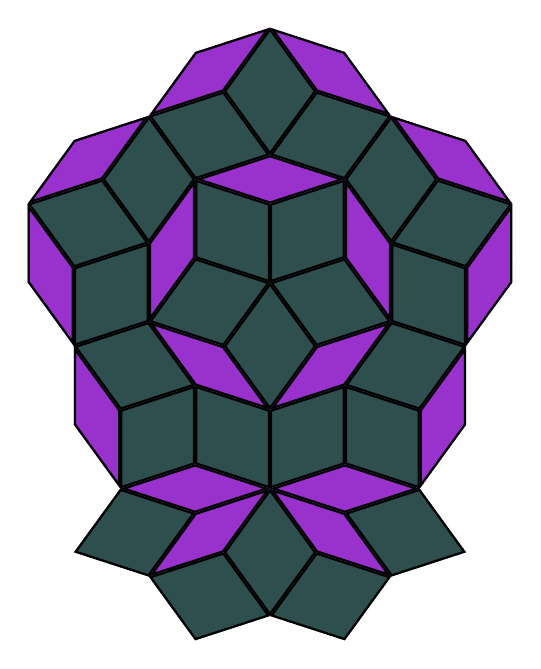
\begin{tikzpicture}[
  every rhombus/.style={
    draw=black,
    ultra thick,
  },
  every thin rhombus/.style={
    every rhombus/.try,
    fill=thinRhombus,
  },
  every thick rhombus/.style={
    every rhombus/.try,
    fill=thickRhombus,
  },
  every circle arc/.style={
    draw=circleArc
  },
  every long arc/.style={
    draw=longArc
  }
]
\pic[rotate=18,thick rhombus,name=a0];
\foreach[evaluate=\k as \kmo using int(\k-1)] \k in {1,...,4} 
{
  \pic[thick rhombus,name=a\k,align with={a\kmo} along A];
}
\foreach \k in {0,...,4} 
{
  \pic[thin rhombus,name=b\k,align with={a\k} along B];
  \pic[thick rhombus,name=c\k,align with={b\k} along A];
  \pic[thick rhombus,name=d\k,align with={b\k} along a];
  \pic[thick rhombus,name=e\k,align with={c\k} along A];
  \foreach \l/\a in {{0/b},{1/B}}
    \pic[thin rhombus,name=f\k\l,align with={e\k} along \a];
}
\pic[thin rhombus,name=g0,align with={f10} along a];
\pic[thin rhombus,name=g1,align with={f21} along A];
\foreach \l/\a in {{0/a},{1/A}}
  \pic[thick rhombus,name=h\l,align with={g\l} along \a];
\pic[thick rhombus,name=i,align with=g0 along B];
\foreach \l/\a in {{0/a},{1/A}}
  \pic[thick rhombus,name=j\l,align with=i along \a];
\end{tikzpicture}
\end{example}

\subsection{Styling}

The tiles can be styled, either directly or using various keys.
When a tile is placed then there are various actions that happen with associated keys.
The actions and keys are:
%
\begin{enumerate}
\item A scope is started and the following keys are tried.
%
\begin{enumerate}
\item \Verb+every tile scope+
\item \Verb+every <name> scope+ where \Verb+name+ is the tile name (not the pic name)
\item \Verb+this tile scope+
\end{enumerate}

\item The tile path is used with the intention of it being a clipping path.
The keys for this action are:
%
\begin{enumerate}
\item \Verb+every tile clip+ by default this is set to \Verb+clip+
\item \Verb+every <name> clip+
\item \Verb+this tile clip+
\end{enumerate}

\item A set of keys are used to allow arbitrary code to be executed before the tile path is rendered.
These are:

\begin{enumerate}
\item \Verb+every tile before path+
\item \Verb+every <name> before path+
\item \Verb+this tile before path+
\end{enumerate}

\item The tile path is rendered.
The keys for this action are:
%
\begin{enumerate}
\item \Verb+every tile+
\item \Verb+every <name>+
\item \Verb+this tile+
\item \Verb+pic actions+
\end{enumerate}

\item A set of keys are used to allow arbitrary code to be executed after the tile path is rendered.
These are:

\begin{enumerate}
\item \Verb+every tile after path+
\item \Verb+every <name> after path+
\item \Verb+this tile after path+
\end{enumerate}
\end{enumerate}


The \Verb+pic actions+ are any actions given directly to the tile, as in \Verb+\pic[draw,thin rhombus];+.
The kite, dart, and rhombus tiles also have arcs drawn on them which are inserted via the \Verb+every <name> after path+ keys, and these are themselves styled ussing \Verb+every circle arc+ and \Verb+every long arc+.
The names come from the way the arcs look on the rhombus shapes.

One other point is important to note about the tiles.
They are actually clipped against themselves.
This ensures that the tiles do not overstep their bounds and so when placed alongside each other then they do not go over each other.
In practical terms, this means that if drawn then the line width is half that which might be expected (but when placed next to another tile, the two halves combine to the expected width).

\subsection{Placing Tiles Automatically}

There is a way to specify certain tilings using \emph{Lindenmayer systems}.
In brief, this takes a seed pattern and successively applies \emph{substitution rules} which are meant to simulate replacing a tile by smaller versions of it (and others from the same set).
This is implemented for the Penrose tiles and the various clusters related to the aperiodical polykite tile.

The Penrose rules are \emph{positional} in that when replacing a Penrose tile by smaller versions of it the new tiles can be placed solely based on information about the position and orientation of the original tile.
This is true also for the \emph{super cluster} tiles of the aperiodical polykite, but not for the meta cluster or subclusters.

The meta and subclusters work on a different system.
The structure that is built up is that of a \emph{tree} with a root tile.
That root tile is positioned, and then the other tiles are placed next to previously placed tiles.
This is a slower process and can mean that the overall shape is different to what might be expected, but from the user's perspective it is the same.

The user command is one of:
%
\begin{verbatim}
\TilingDecomposition{<type>}{<level>}{<seed>}
\pic{decomposition={<type>}{<level>}{<seed>}};
\end{verbatim}
%
where \Verb+<type>+ is one of:
%
\begin{itemize}
\item \Verb+kite+ for the kite and dart tiling,
\item \Verb+rhombus+ for the rhombus tiling,
\item \Verb+pentagon+ for the pentagon tiling.
\item \Verb+ktriangle+ for the triangular decomposition used to form the kite and dart tiling but with the individual triangles
\item \Verb+rtriangle+ for the triangular decomposition used to form the rhombus tiling but with the individual triangles.
\item \Verb+supercluster+ for the super cluster substitution system that works on a positional basis.
\item \Verb+cluster+ for the cluster substitution system that uses the neighbour information.
The choice of super, meta, or subcluster is determined by the value of the key \Verb!cluster type!.
\end{itemize}

The \Verb+<seed>+ is a ``word'' that will be used to initiate the Lindenmayer system.
The key letters in the alphabet for the kite/darts and rhombuses are \Verb+T+, \Verb+t+, \Verb+G+, and \Verb+g+.
These actually correspond to the two triangles and two gnomons.
For the pentagons, the key letters are \Verb+P+, \Verb+Q+, \Verb+R+, \Verb+G+, \Verb+B+, \Verb+D+.
These correspond to the three pentagons, the pentagram, the boat, and the diamond.
For the clusters, the key letters are \Verb+H+, \Verb+T+, \Verb+P+, and \Verb+F+.
Other permitted letters are \Verb+[+, \Verb+]+, \Verb+s+, \Verb+f+, \Verb!+!, \Verb+*+, \Verb+-+, \Verb+_+, \Verb+>+.
These refer to various transformations (for details, see the implementation).

The \Verb+<level>+ controls how far to take the iteration.
The code is not particularly optimised for speed, and once \Verb+<level>+ gets to about \(5\) or \(6\) then we are at the ``make a cup of tea while compiling'' stage, depending on the processor.

\begin{example}
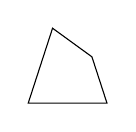
\begin{tikzpicture}[
  every tile/.style={draw},
  step=2cm,
]
\TilingDecomposition{kite}{0}{T}
\end{tikzpicture}
\end{example}

The two types of substitution rules -- positional and neighbourly -- are rendered slightly differently.
The positional tiles are drawn directly but the neighbour ones are drawn via the \Verb!\pic! mechanism.
This is to exploit the existing code for aligning against existing tiles.
This means that the \Verb!\pic! styling options are available for the latter type of decomposition but not for the former.
For the former, only the following keys are used:

\begin{verbatim}
every tile
every <tile type>
\end{verbatim}

There are, however, some additional styles which allow styling the tiles by their number: a count is kept of the number of tiles and each tile knows its own number.
Specifically, two keys are tried:
%
\begin{enumerate}
\item \Verb+tile <number>+, and
\item \Verb+tile={<number>}{<total>}+
\end{enumerate}
%
A word of warning is in order on the second of these.
The \Verb+<total>+ is not guaranteed to be correct.
It is done by a quick count at the start of the process and counts those letters which \emph{might} result in a rendered tile.
Not every letter in the resulting word actually does.
Nevertheless, this can be used to style a tile based on what proportion of tiles have been rendered.

Lastly, \Verb+step+ is used to control the size of the resulting picture.

\begin{example}
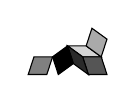
\begin{tikzpicture}[
  every tile/.style={draw},
  step=4cm,
  tile/.code 2 args={
    \pgfmathsetmacro\tint{100*#1/#2}
    \pgfkeysalso{fill=black!\tint}
  }
]
\TilingDecomposition{rhombus}{3}{T}
\end{tikzpicture}
\end{example}


\section{Deforming Paths}
\label{sec:pathdeform}

This package provides the ability to deform the edges of the tiles.
The tiles are built from labelled paths together with their reverses.
By changing these paths, one can get a wide variety of different tiles with the same fundamental matching rules.
Indeed, by using asymmetric paths, the matching rules can be enforced without the need for additional decoration.

Internally, the \Verb+tiling+ library uses the \Verb+spath3+ package for storing and manipulating the paths.

To create a new edge path, use the key \Verb+save tiling path=<edge>+ where \Verb+<edge>+ is a symbol used in the edge description of a tile.
There are no constraints on the size of the path as all paths are scaled and transformed to fit the tiles.
Once the edge paths have been specified, they are welded together into the tiles using the following command:
%
\begin{verbatim}
\BakeTile{<name>}
\end{verbatim}
%
Here, \Verb+<name>+ is one of the names of the tiles.
This has global effect, as does the definition of the edge paths.
Paths, both sides and tiles, can be cloned via:
%
\begin{verbatim}
\tikzset{clone tiling side path={target}{source}}
\tikzset{clone tile path={target}{source}}
\end{verbatim}
%
and restored with the same command (but names switched).

\begin{example}
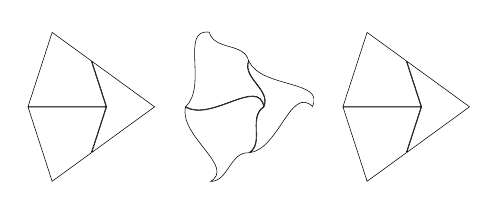
\begin{tikzpicture}
\pic[draw,dart,name=dart];
\pic[draw,kite,align with=dart along c];
\pic[draw,kite,align with=dart along C];
\tikzset{clone tile path={original kite}{kite}}
\tikzset{clone tile path={original dart}{dart}}
\path[save tiling path=a] (0,0) to[out=-30,in=100] (1,0);
\path[save tiling path=c] (0,0) to[out=-40,in=140] (1,0);
\BakeTile{kite}
\BakeTile{dart}
\pic[xshift=2cm,draw,dart,name=dart];
\pic[draw,kite,align with=dart along c];
\pic[draw,kite,align with=dart along C];
\tikzset{clone tile path={kite}{original kite}}
\tikzset{clone tile path={dart}{original dart}}
\pic[xshift=4cm,draw,dart,name=dart];
\pic[draw,kite,align with=dart along c];
\pic[draw,kite,align with=dart along C];
\end{tikzpicture}
\end{example}

With deformed tiles there is no guarantee that the inner arcs on the Penrose tiles will match up perfectly.

Note that the subcluster tiles from the polykite subpackage are actually already deformed tiles.

\begin{example}
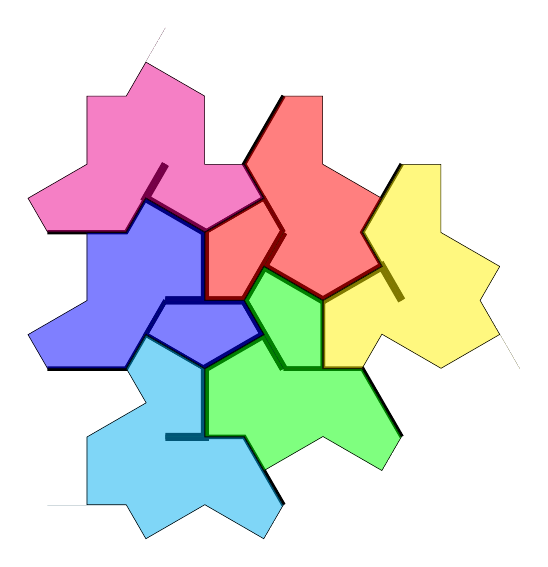
\begin{tikzpicture}[
  every subcluster F/.style={draw, ultra thick},
  every subcluster P/.style={draw, thick},
  every subcluster H/.style={draw, fill, fill opacity=.5}
]
\pic[subcluster F, name=F1, this tile/.style={line width=1mm}];
\pic[subcluster F, align with=F1 along 12 using 1, name=F2, this tile/.style={line width=1mm}];
\pic[subcluster F, align with=F1 along 11 using 2, name=F3, this tile/.style={line width=1mm}];
\pic[subcluster F, align with=F1 along F,name=F1-2];
\pic[subcluster F, align with=F1 along f,name=F1-3];
\pic[subcluster F, align with=F2 along F,name=F2-2];
\pic[subcluster F, align with=F2 along f,name=F2-3];
\pic[subcluster F, align with=F3 along F,name=F3-2];
\pic[subcluster F, align with=F3 along f,name=F3-3];
\pic[subcluster H, align with=F1 along b using 2, fill=red];
\pic[subcluster H, align with=F2 along b using 2, fill=green];
\pic[subcluster H, align with=F3 along b using 2, fill=blue];
\pic[subcluster H, align with=F1-2 along b using 1, fill=yellow];
\pic[subcluster H, align with=F2-2 along b using 1, fill=cyan];
\pic[subcluster H, align with=F3-2 along b using 1, fill=magenta];
\end{tikzpicture}
\end{example}

\begin{example}
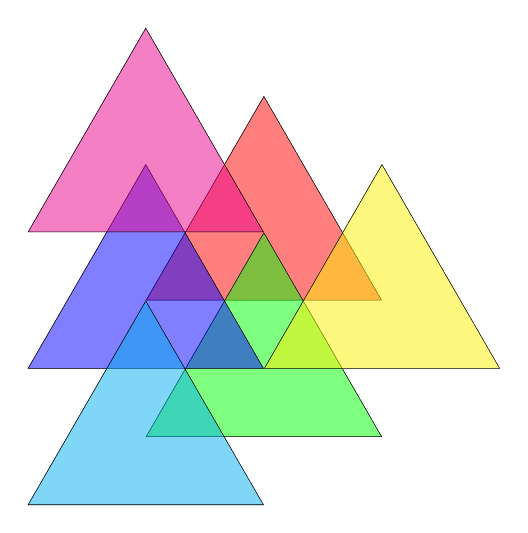
\begin{tikzpicture}[
  every tile pic/.style={},
%  every subcluster F/.style={draw, ultra thick},
%  every subcluster P/.style={draw, thick},
  every subcluster H/.style={draw, fill, fill opacity=.5}
]
\path[save tiling path=a] (0,0) -- (1,0);
\path[save tiling path=b] (0,0) -- (1,0);
\path[save tiling path=f] (0,0) -- (1,0);
\BakeTile{subcluster H}
\BakeTile{subcluster T}
\BakeTile{subcluster P}
\BakeTile{subcluster F}

\pic[subcluster F, name=F1, this tile/.style={line width=1mm}];
\pic[subcluster F, align with=F1 along 12 using 1, name=F2, this tile/.style={line width=1mm}];
\pic[subcluster F, align with=F1 along 11 using 2, name=F3, this tile/.style={line width=1mm}];
\pic[subcluster F, align with=F1 along F,name=F1-2];
\pic[subcluster F, align with=F1 along f,name=F1-3];
\pic[subcluster F, align with=F2 along F,name=F2-2];
\pic[subcluster F, align with=F2 along f,name=F2-3];
\pic[subcluster F, align with=F3 along F,name=F3-2];
\pic[subcluster F, align with=F3 along f,name=F3-3];
\pic[subcluster H, align with=F1 along b using 2, fill=red];
\pic[subcluster H, align with=F2 along b using 2, fill=green];
\pic[subcluster H, align with=F3 along b using 2, fill=blue];
\pic[subcluster H, align with=F1-2 along b using 1, fill=yellow];
\pic[subcluster H, align with=F2-2 along b using 1, fill=cyan];
\pic[subcluster H, align with=F3-2 along b using 1, fill=magenta];
\end{tikzpicture}
\end{example}

\section{More Examples}

Let's set some aesthetically pleasing shapes.
Note that I'm using the TikZ \Verb!external! library in creating this document so to deform the paths in the examples I need to add the deformation code to every picture (otherwise the externalisation skips it).
I've saved it into a key \Verb!deform tiles! to avoid overwhelming the example code.
In a document without externalisation then adding the following code will achieve the same effect.

\begin{justexample}
\begin{tikzpicture}
\path[save tiling path=a] (0,0) to[out=-30,in=100] (1,0);
\path[save tiling path=b] (0,0) to[out=0,in=140] (1,0);
\path[save tiling path=c] (0,0) to[out=-40,in=140] (1,0);
\BakeTile{thin rhombus}
\BakeTile{thick rhombus}
\BakeTile{golden triangle}
\BakeTile{reverse golden triangle}
\BakeTile{golden gnomon}
\BakeTile{reverse golden gnomon}
\BakeTile{kite}
\BakeTile{dart}
\end{tikzpicture}
\end{justexample}

\tikzset{
  deform tiles/.code={%
    \path[save tiling path=a] (0,0) to[out=-30,in=100] (1,0);
    \path[save tiling path=b] (0,0) to[out=0,in=140] (1,0);
    \path[save tiling path=c] (0,0) to[out=-40,in=140] (1,0);
    \BakeTile{thin rhombus}
    \BakeTile{thick rhombus}
    \BakeTile{golden triangle}
    \BakeTile{reverse golden triangle}
    \BakeTile{golden gnomon}
    \BakeTile{reverse golden gnomon}
    \BakeTile{kite}
    \BakeTile{dart}
  }
}

Styling the first tile.
Note that as the pattern is formed by repeating two different initial seeds \(5\) times, there are \(10\) ``first tiles'' in each overall pattern.

\begin{example}
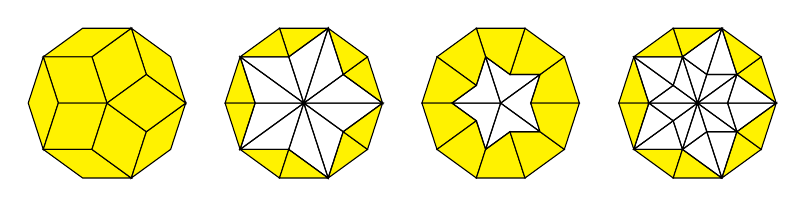
\begin{tikzpicture}[
  deform tiles/.try,
  every tile/.style={draw},
  tile 1/.style={fill=yellow},
]
\foreach \tp/\pos in {rhombus/0cm,rtriangle/2.5cm,kite/5cm,ktriangle/7.5cm}
{
\begin{scope}[xshift=\pos]
\foreach[evaluate=\k as \mk using {\k+Mod(\k,2)},evaluate=\k as \ax using {Mod(\k,2) == 0 ? "T" : "t"}] \k in {0,...,9} {
  \begin{scope}[rotate=\mk*36]
  \TilingDecomposition{\tp}{1}{\ax}
  \end{scope}
}
\end{scope}
}
\end{tikzpicture}
\end{example}



A more detailed decomposition, with more and more tinting applied to each tile.
Roughly half of the counted tiles are rendered, and the ordering in which they are rendered is not at first an obvious one (though it is in general from ``outside in'').

Note that the key \Verb+tint fill colour+ is not a TikZ native.
It is defined as:

\begin{verbatim}
\makeatletter
\tikzset{
  tint fill colour/.code={%
    \edef\@temp{%
      \def\noexpand\tikz@fillcolor{\tikz@fillcolor!#1}%
      \noexpand\tikz@addoption{%
        \noexpand\pgfsetfillcolor{\tikz@fillcolor!#1}%
      }%
    }%
    \@temp
  }
}
\makeatother
\end{verbatim}

\begin{example}
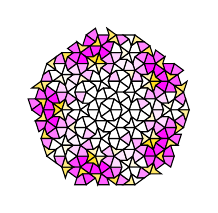
\begin{tikzpicture}[
  deform tiles/.try,
  every tile/.style={draw},
  every kite/.style={fill=reverseGoldenTriangle},
  every dart/.style={fill=goldenTriangle},
  tile/.code 2 args={
    \pgfmathsetmacro\tint{100*(1 - 1.5*#1/#2))}
    \pgfkeysalso{tint fill colour=\tint}
  }
]
\foreach[evaluate=\k as \mk using {\k+Mod(\k,2)},evaluate=\k as \ax using {Mod(\k,2) == 0 ? "T" : "t"}] \k in {0,...,9} {
  \begin{scope}[rotate=\mk*36]
  \TilingDecomposition[step=5cm]{kite}{4}{\ax}
  \end{scope}
}
\end{tikzpicture}
\end{example}

An example with ``manual placement''.

\begin{example}
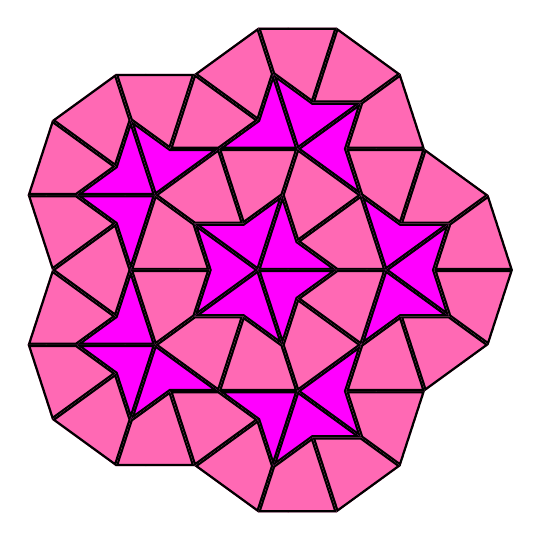
\begin{tikzpicture}[
  deform tiles/.try,
  every tile/.style={
    draw=black,
    ultra thick,
  },
  every kite/.style={
    fill=kite,
  },
  every dart/.style={
    fill=dart,
  },
  every circle arc/.style={
    draw=circleArc
  },
  every long arc/.style={
    draw=longArc
  }
]
\pic[dart,name=a0];
\foreach[evaluate=\k as \kmo using int(\k-1)] \k in {1,...,4} {
  \pic[dart,name=a\k,align with={a\kmo} along a];
}
\foreach \k in {0,...,4} {
  \foreach \l/\e/\ee in {0/c/a,1/C/A} {
    \pic[kite,name=b\l\k,align with={a\k} along \e];
    \pic[dart,name=c\l\k,align with={b\l\k} along \ee];
    \pic[kite,name=d\l\k,align with={c\l\k} along \e];
  }
  \pic[kite,name=e\k,align with={c0\k} along C];
  \pic[dart,name=f\k,align with={c0\k} along a];
  \foreach \e in {c,C} {
    \pic[kite,name=g\k,align with={f\k} along \e];
  }
}
\end{tikzpicture}
\end{example}


The decomposition rules for the Lindenmayer system can be illustrated by drawing each tile together with the result of one decomposition superimposed on top.

\begin{example}
\foreach \ax in {T,t,G,g} {

\begin{tikzpicture}[
  deform tiles/.try,
]
\foreach \tp/\pos in {rhombus/0cm,rtriangle/2cm,kite/4cm,ktriangle/6cm}
{
\begin{scope}[xshift=\pos]
  \TilingDecomposition[every path/.style={draw=red,ultra thick}]{\tp}{0}{\ax}
  \TilingDecomposition[every path/.style={fill=gray!50,fill opacity=.5,draw=black}]{\tp}{1}{\ax}
\end{scope}
}
\end{tikzpicture}

}
\end{example}

The tiles can make interesting forms by themselves.

\begin{example}
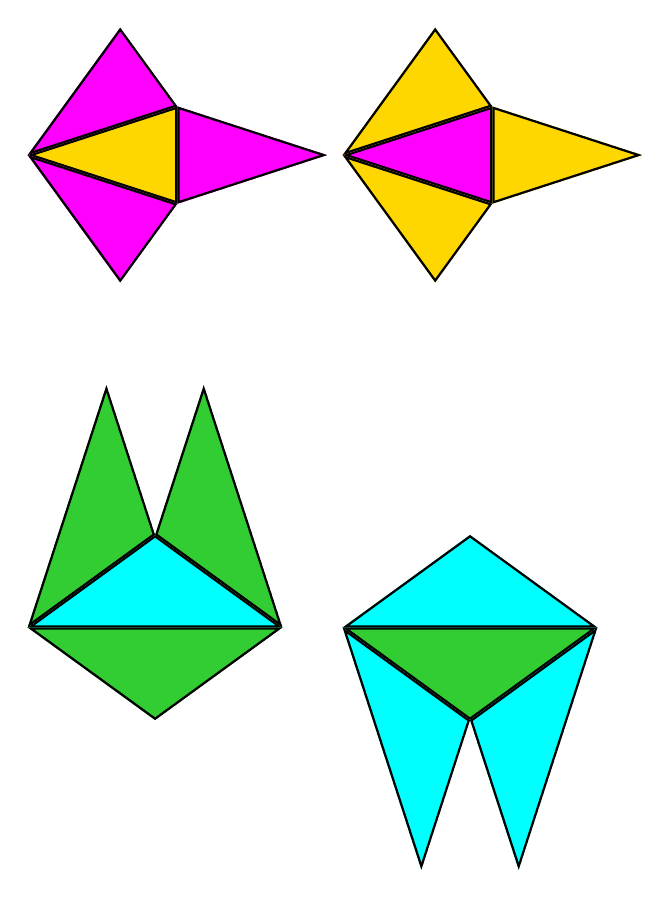
\begin{tikzpicture}[
  deform tiles/.try,
  scale=2,
  every tile pic/.style={
    transform shape,
  },
  every golden triangle/.style={
    draw=black,
    ultra thick,
    fill=goldenTriangle,
  },
  every reverse golden triangle/.style={
    draw=black,
    ultra thick,
    fill=reverseGoldenTriangle,
  },
  every golden gnomon/.style={
    draw=black,
    ultra thick,
    fill=goldenGnomon,
  },
  every reverse golden gnomon/.style={
    draw=black,
    ultra thick,
    fill=reverseGoldenGnomon,
  },
]
\pic[golden triangle,name=a];
\pic[reverse golden triangle,align with=a along a];
\pic[reverse golden triangle,align with=a along b];
\pic[reverse golden triangle,align with=a along c];
\begin{scope}[xshift=2cm]
\pic[reverse golden triangle,name=a];
\pic[golden triangle,align with=a along A];
\pic[golden triangle,align with=a along B];
\pic[golden triangle,align with=a along C];
\end{scope}
\begin{scope}[yshift=-3cm]
\pic[golden gnomon,name=a];
\pic[reverse golden gnomon,align with=a along C];
\pic[reverse golden gnomon,align with=a along b];
\pic[reverse golden gnomon,align with=a along A];
\begin{scope}[xshift=2cm]
\pic[reverse golden gnomon,name=a];
\pic[golden gnomon,align with=a along c];
\pic[golden gnomon,align with=a along B];
\pic[golden gnomon,align with=a along a];
\end{scope}
\end{scope}
\end{tikzpicture}
\end{example}

\begin{example}
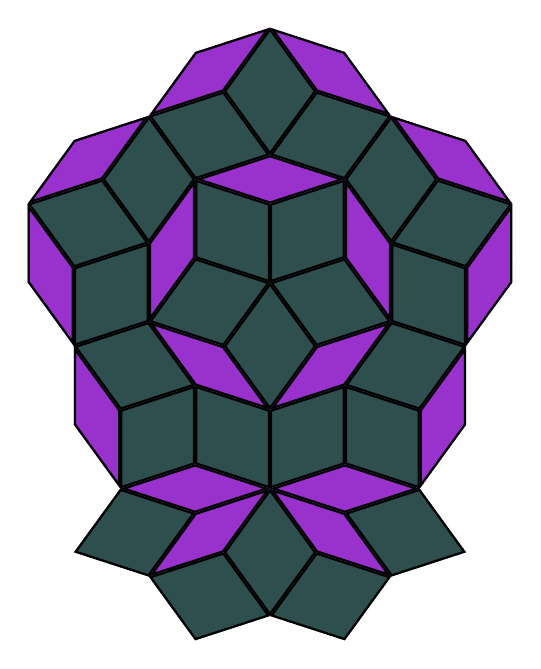
\begin{tikzpicture}[
  deform tiles/.try,
  every rhombus/.style={
    draw=black,
    ultra thick,
  },
  every thin rhombus/.style={
    every rhombus/.try,
    fill=thinRhombus,
  },
  every thick rhombus/.style={
    every rhombus/.try,
    fill=thickRhombus,
  },
  every circle arc/.style={
    draw=circleArc
  },
  every long arc/.style={
    draw=longArc
  }
]
\pic[rotate=18,thick rhombus,name=a0];
\foreach[evaluate=\k as \kmo using int(\k-1)] \k in {1,...,4} 
{
  \pic[thick rhombus,name=a\k,align with={a\kmo} along A];
}
\foreach \k in {0,...,4} 
{
  \pic[thin rhombus,name=b\k,align with={a\k} along B];
  \pic[thick rhombus,name=c\k,align with={b\k} along A];
  \pic[thick rhombus,name=d\k,align with={b\k} along a];
  \pic[thick rhombus,name=e\k,align with={c\k} along A];
  \foreach \l/\a in {{0/b},{1/B}}
    \pic[thin rhombus,name=f\k\l,align with={e\k} along \a];
}
\pic[thin rhombus,name=g0,align with={f10} along a];
\pic[thin rhombus,name=g1,align with={f21} along A];
\foreach \l/\a in {{0/a},{1/A}}
  \pic[thick rhombus,name=h\l,align with={g\l} along \a];
\pic[thick rhombus,name=i,align with=g0 along B];
\foreach \l/\a in {{0/a},{1/A}}
  \pic[thick rhombus,name=j\l,align with=i along \a];
\end{tikzpicture}
\end{example}

Lastly, here's an example that generates full page patterns.

\begin{justexample}
\foreach \tp/\lvl in {rhombus/5,rhombus/6,kite/5,kite/6}
{
\tikzset{external/export next=false}
\begin{tikzpicture}[
  every tile/.style={draw},
  remember picture,
  overlay,
  scale=20
]
\coordinate (a) at (current page.center);
\begin{scope}[shift={(a)}]
\foreach[evaluate=\k as \mk using {\k+Mod(\k,2)},evaluate=\k as \ax using {Mod(\k,2) == 0 ? "T" : "t"}] \k in {0,...,9} {
  \begin{scope}[rotate=\mk*36]
  \TilingDecomposition{\tp}{\lvl}{\ax}
  \end{scope}
}
\end{scope}
\end{tikzpicture}
\newpage
}
\end{justexample}
\end{document}

\begin{tikzpicture}
\path[save tiling path=a] (0,0) -- (1,0);
\path[save tiling path=b] (0,0) -- (1,0);
\path[save tiling path=c] (0,0) -- (1,0);
\BakeTile{thin rhombus}
\BakeTile{thick rhombus}
\BakeTile{golden triangle}
\BakeTile{reverse golden triangle}
\BakeTile{golden gnomon}
\BakeTile{reverse golden gnomon}
\BakeTile{kite}
\BakeTile{dart}
\end{tikzpicture}

\newpage

\foreach \tp/\lvl in {rhombus/5,rhombus/6,kite/5,kite/6}
{
\begin{tikzpicture}[
  every tile/.style={draw},
  remember picture,
  overlay,
  scale=20
]
\coordinate (a) at (current page.center);
\begin{scope}[shift={(a)}]
\foreach[evaluate=\k as \mk using {\k+Mod(\k,2)},evaluate=\k as \ax using {Mod(\k,2) == 0 ? "T" : "t"}] \k in {0,...,9} {
  \begin{scope}[rotate=\mk*36]
  \TilingDecomposition{\tp}{\lvl}{\ax}
  \end{scope}
}
\end{scope}
\end{tikzpicture}
\newpage
}


%% \foreach \lvl in {5,6}
%% {
%% \begin{tikzpicture}[
%%   every tile/.style={draw},
%%   remember picture,
%%   overlay,
%%   scale=180
%% ]
%% \coordinate (a) at (current page.center);
%%   \TilingDecomposition{pentagon}{\lvl}{D}
%% \end{tikzpicture}
%% \newpage
%% }


\end{document}

% Local Variables:
% tex-output-type: "pdf18"
% End:
